\chapter{Introduction}
\label{ch:intro}

\section{Motivation}
\label{sec:motivation}

Debugging is a task that every developer and software engineer will have to go
through while writing code. It's often a
tedious process that involves manually checking the code and running it multiple
times to simply find the location of the error in the code. More formally,
debugging ``involves analyzing and possibly extending the given program that
does not meet the specification in order to find a new program that is close to
the original and does satisfy the specifications... it is the process of
`diagnosing the precise nature of a known error and then correcting it' '' \cite{Hailpern2002Debugging}.
Finding possible solutions to fix the fault would then be the next step
in the debugging process. In Postman's 2020 State of the API Report,
developers reported allocating seventeen percent of their time
debugging and manually testing their code.
Fig \ref{fig:development_time} demonstrates that debugging makes up the
second most time-consuming task for API developers.
In an effort to facilitate and automate this process, different tools have been
created to guide the developer in locating error(s) and suggesting how to go
about fixing them. Solving this problem can significantly increase the
efficiency of experienced developers and increase the quality of the code they
ship. Additionally, a solution can help in decreasing the time spent on
debugging and allow developers to focus on other important tasks.
Beginner and novice developers can also benefit greatly from tools
that facilitate the debugging process, which could ease the learning process and help
them avoid making mistakes. Overall, contributions to this field of study could
assist developers and software engineers of all levels.
With special concentration on novice and beginner developers in an educational
environment, this research implements and evaluates a tool focused on helping
developers find bugs in their code.

% TODO: check all citations
% TODO: create citation
\begin{figure}[!htb]
	\begin{center}
		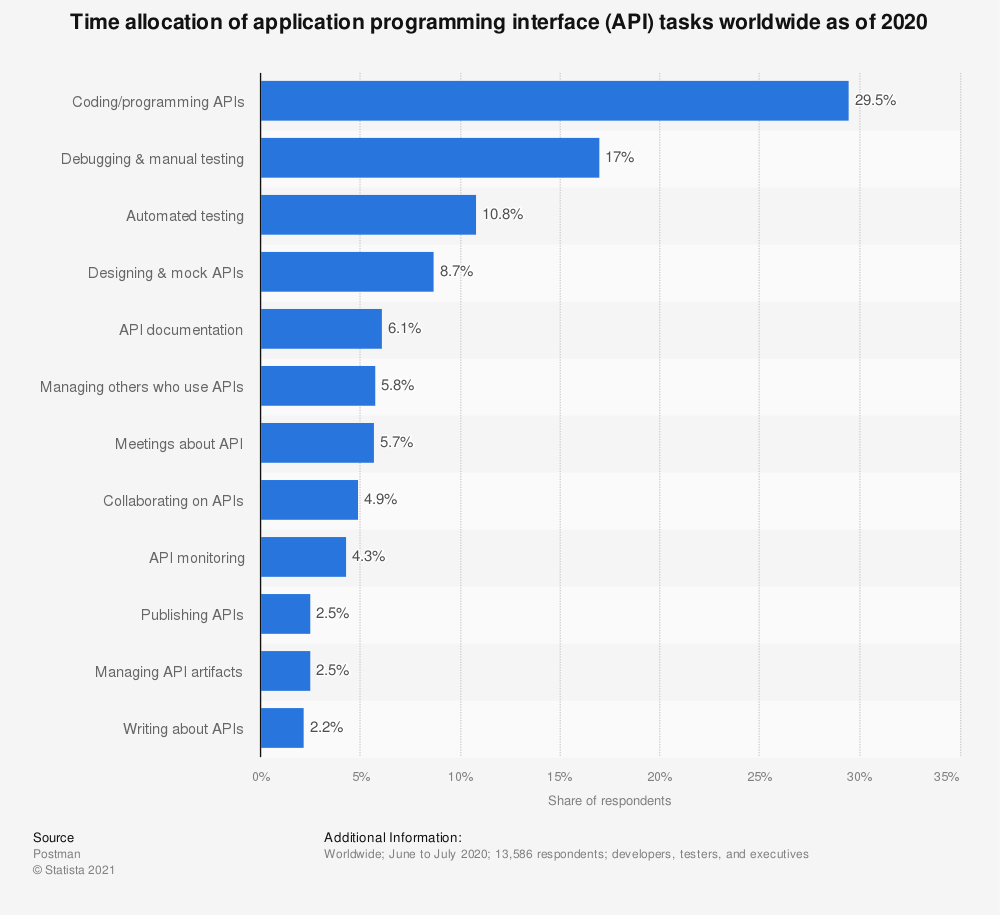
\includegraphics[width=\textwidth]{dev_time_stat.png}
		\caption{\label{fig:development_time} API Developers Time Allocation}
	\end{center}
\end{figure}

\section{Background}
\label{sec:background}

\subsection{Debugging and Fault Localization}
\label{subsec:DebuggingAndAFL}

The debugging process for developers typically starts when a ``bug'',
unexpected/incorrect behavior has been observed. One of many ways to check
whether incorrect behavior is taking place is through unit testing. This type of
testing consists of a set of test cases that check the different functionalities of the
code by asserting that expected output and actual output match. When a test case
fails due to a mismatch in the assertion, the search for the causing bug begins.
This research focuses on this crucial step in debugging and aims to guide the
search process by setting priority locations for the developers to search in.

Debugger tools have often been used to find and fix bugs in code, and while they
have several benefits, they also have drawbacks. Debuggers provide the developer
with a way to essentially pause the runtime of a program using breakpoints to display
information about the state of different variables and function call stack.
Through debuggers, developers can run the code line by line until an unexpected
behavior is detected. There is no denial that debuggers are very effective,
however, using them can be time-consuming, especially for complex bugs.
Additionally, debuggers require that the code is run during the debugging
process which could increase the time needed to debug and might not always be
feasible. With these drawbacks in mind, several automated fault localization (AFL)
algorithms and approaches have been studied to increase the
efficiency of the debugging process.

% TODO: find the sources that explores different types of AFL
Automated Fault Localization approaches perform different types of analysis to
the code and attempt to find the location of existing faults. Some approaches
use trained artificial intelligence models to assess the code and make
predictions on where some faults may exist. Others construct and analyze
abstract syntax trees to look for potential errors. On the other hand,
approaches such as spectrum-based fault localization rely on data collected
during the runtime of the code to ``identify the part of the program whose
activity correlates most with the detection of errors'' \cite{ABREU20091780}.
More specifically, the results of the program's test suite are used to find this
correlation. This latter approach is the focus of this research, where a
spectrum-based automated fault localization tool is implemented.

\subsection{Spectrum Based Fault Localization}
\label{subsec:SpectrumBased}

The reliance of spectrum based fault localization (SBFL) on data already
collected during running and testing reduces the overall cost of debugging since
there is no need to rerun the code. When focusing on collected test suite data,
SBFL becomes even more applicable since it can be integrated with many unit test
frameworks. In addition to the per-test outcome of a test suite, per-test
coverage data is also used in SBFL to identify which lines are executed by each
test case. Once this data is collected following a test suite run, SBFL assesses
the suspiciousness of code blocks depending on how many failing test cases run
those blocks. From a logical point of view, the block/line of code executed the
most by a failing test case is the most likely to contain the fault. SBFL also
uses various equations to calculate and quantify the
suspiciousness of blocks of code. The equations are expressed as functions of
elements, where each element is the line or block of code under inspection. The
functions typically include the variables shown in
Fig.\ref{fig:contingency_table}. The figure also provides a table to visualize
the relationship of the variables \cite{Wong2014DStar}.

\begin{figure}[!htb]
	\begin{center}
		\textbf{N$_{CF}$}: number of failed test cases that execute/cover the element

		\textbf{N$_{UF}$}: number of failed test cases that do not execute/cover the element
	
		\textbf{N$_{CS}$}: number of passed test cases that execute/cover the element
	
		\textbf{N$_{US}$}: number of passed test cases that do not execute/cover the element
		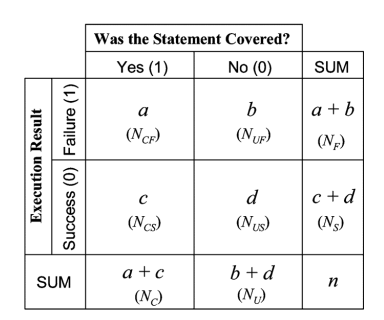
\includegraphics[width=7cm]{contingency_table.png}
		\caption{\label{fig:contingency_table} Variables in SBFL}
	\end{center}
\end{figure}

% TODO: needs updated when the fourth equation is picked
Using these variables, past research has come up with many equations to
calculate elements' suspiciousness scores. This research focuses on three main
popular equations and adds support for them in AFLuent. The reasoning behind the
equation choices is further discussed in Related Works, however, this section
will give an overview of how each looks like.

\subsubsection{Tarantula}
\label{subsubsec:Tarantula}
\begin{figure}[!htb]
	\begin{center}
		\begin{equation}
			Tarantula(element) = \frac{\frac{\textbf{N$_{CF}$}}{\textbf{N$_{CF}$} + \textbf{N$_{UF}$}}}{\frac{\textbf{N$_{CS}$}}{\textbf{N$_{CS}$}+\textbf{N$_{US}$}} + \frac{\textbf{N$_{CF}$}}{\textbf{N$_{CF}$}+\textbf{N$_{UF}$}}}
		\end{equation}
		\caption{\label{fig:tarantulaEquation} Tarantula Equation\cite{Jones2005TarantulaEval}}
	\end{center}
\end{figure}

The Tarantula equation is one of the most popular Coverage based fault localization
formulas to calculate suspiciousness scores of code elements. It uses the
variables listed previously to generate a score between 0 and 1, where 0 is
assigned for non-suspicious elements and 1 is assigned for most suspicious ones.

\subsubsection{Ochiai}
\label{subsubsec:Ochiai}
\begin{figure}[!htb]
	\begin{center}
		\begin{equation}
			Ochiai(element) = \frac{\textbf{N$_{CF}$}}{\sqrt{(\textbf{N$_{CF}$}  + \textbf{N$_{UF}$}) \cdot (\textbf{N$_{CF}$}  + \textbf{N$_{CS}$})}}
		\end{equation}
		\caption{\label{fig:ochiaiEquation} Ochiai Equation\cite{Abreu2006Ochiai}}
	\end{center}
\end{figure}

Ochiai is another equation used to calculate suspiciousness scores between 0 and
1. It relies on similar code test and coverage variables as the Tarantula
equation. AFLuent supports using this equation in its automated fault
localization process. More discussion around Ochiai can be found in the related
works section.

\subsubsection{DStar}
\label{subsubsec:DStar}
\begin{figure}[!htb]
	\begin{center}
		\begin{equation}
			Dstar(element) = \frac{(\textbf{N$_{CF}$})^{\ast}}{\textbf{N$_{CS}$} + \textbf{N$_{UF}$}}
		\end{equation}
		\caption{\label{fig:dstarEquation} DStar Equation\cite{Wong2014DStar}}
	\end{center}
\end{figure}

The scores resulting from the DStar equation can range beyond 0 and 1 because it includes
a new variable represented as the * symbol. This variable can give more
weight to \textbf{N$_{CF}$} and can be set to any number. However, the
researchers suggested that * is set to 2 or 3.

\subsection{SBFL in Action}
\label{subsec:SBFLinAction}

\begin{figure}[!htb]
	\begin{center}
		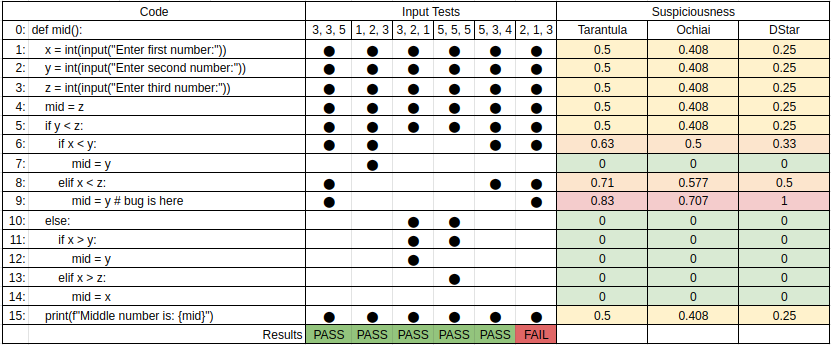
\includegraphics[width=\textwidth]{SFL_example.png}
		\caption{\label{fig:sbfl_example} Applied Example of SBFL Equations}
	\end{center}
\end{figure}

With the discussed equations and techniques to calculate suspiciousness in mind,
the following example will demonstrate and discuss how AFLuent will utilize unit
test and coverage data to locate faults in a program.
Fig.\ref{fig:sbfl_example}
shows a sample python program to find the middle value
from three integers. The program contains a bug on line 9 where the wrong middle
number is detected. The figure also shows six different test cases that pass
various inputs to the function and check whether the actual output matches the
expected. The results of each test is found on the last row of the table.
Additionally, the large dots under the Input Tests column illustrate the concept
of code coverage. For each line of code and test input, a dot in the cell means
that the line was executed when this input was passed. On the rightmost column
of the table, suspiciousness scores for each line are calculated using the three
formulas (Tarantula, Ochiai, and DStar). High suspiciousness scores are also
highlighted in warmer colors. Overall, all three equations are able to detect
that line 9 is the most suspicious and is likely the cause of the test failure.

\subsection{SBFL Criticism}
\label{subsec:Criticism}

While SBFL can provide great insight for developers looking to debug their code,
it's not always reliable or applicable. In the case where a test suite hasn't
been fully implemented, the output of SBFL may not narrow down potentially faulty
code to a single line. Additionally, ties in suspiciousness scores between lines
and blocks may come up, which may not offer the developer any valuable output.
Overall limitations of SBFL will be discussed in Related Works and acknowledged
while evaluating the outcome of this research.

\section{Main Aims}
\label{sec:aims}

% TODO: maybe talk about the other existing python tool?
With the demonstrated importance of debugging tools and strategies that increase
developer efficiency, this research implements and evaluates an AFL tool to
assist in debugging code. AFLuent is built using  Python programming
language and uses SBFL approach to identify faults in a
% TODO: create citation
program. Stack Overflow 2021 Developer Survey identified Python as the third
most used programming/markup language used by developers worldwide. With that in
mind, an automated fault localization tool in Python can reach a wide audience
in various fields such as data science and AI who may have various levels of
experience. By implementing AFLuent using Python, powerful libraries and
packages such as Pytest and Coverage.py can be used to collect test suite data
in order to calculate suspiciousness. AFLuent runs as a Pytest plugin and is
integrated with the command line interface of Pytest, this feature increases
it's accessibility by allowing developers to easily integrate it into their
development environment.

Following the implementation of AFLuent, this research evaluates the
tool's performance and accuracy. Several open source projects
available on GitHub are handpicked to run AFLuent against. A representative
sample of projects with various sizes and relevance will be used to collect
data. Mutation testing libraries are used to introduce bugs into the code,
following that step, AFLuent uses the resulting test suite data to identify the
introduced fault. Through this process, AFLuent's performance and ability to
correctly identify and rank suspicious statements/and blocks assessed.
The evaluation section will describe this crucial process that ensures that
AFLuent functions as intended and is able to locate faults in code.

\section{Research Questions}
\label{sec:researchq}

Throughout the implementation, testing, and evaluation of AFLuent, this research
presents the following research questions and aims to answer each in detail.
There are two main research questions that focus on different aspects of
AFLuent. Each one is further split into sub-questions to facilitate organization.

\begin{center}
	\emph{RQ1. What are the most accurate available techniques to automate the process of
	fault localization using test coverage data?
	}
\end{center}

This general research question focuses on the core implementation and
evaluation of AFLuent. Considering that many SBFL strategies and formulas can be
used, finding the most suitable and most accurate one in detecting bugs is one
of the goals of this research. In order to answer this question,
available literature on SBFL is analysed and the most popular and cited formulas
are included in the implementation of AFLuent. Answering this question also
requires that each approach is evaluated through an experiment section.
Since this research question is includes two separate sections, it's further split into
smaller sub-questions discussed below.

\begin{center}
	\emph{RQ1.1. What are the four most popular formulas for code suspiciousness
	created and evaluated by past literature?
	}
\end{center}

Available literature surrounding SBFL is reviewed to identify four
different formulas used to calculate suspiciousness scores using test coverage
information. Each of these formulas are integrated into AFLuent where the user
is able to select the approach to use while debugging. The popularity, accuracy,
and performance as found in past work are the main criteria used to pick the top
formulas.


\begin{center}
	\emph{RQ1.2.  What is the accuracy and efficiency of the chosen
	formulas when applied to Python projects?
	}
\end{center}

To ensure correctness and effectiveness, the implemented formulas in AFLuent are
evaluated through experiments that measure their accuracy in sorting suspicious
statements and blocks. More specifically, the formulas will be assessed in in
the context of Python projects that use the Pytest unit testing framework.
More details on this research question can be found in the evaluation section.

While RQ1 involves technical details around implementation and assessment of
AFLuent, RQ2 focuses on user experience. Since the target audience of AFLuent is
beginner developers, it's important to ensure that AFLuent produces meaningful
and clear results that guide developers. In order to answer this question,
AFLuent adopts various standards in interacting with the user through console
output, as well as error messages and warnings.

\begin{center}
	\emph{RQ2. How can automated fault localization techniques be implemented in
	Python as a novice developer friendly tool?
	}
\end{center}

In addition to ensuring a smooth user experience while utilizing AFLuent
functionalities, setup process and usage of the tool AFLuent is simplified to
facilitate installation. Clear and descriptive documentation is also a crucial
step in making AFLuent accessible available for new users.

\section{Thesis Outline}
\label{sec:outline}

Starting with a literature review, this research identifies important sources
that guide the implementation of AFLuent and discusses their use. Additionally,
the methods section extensively describes how AFLuent is implemented and the
steps taken to ensure it functions correctly while being up to industry
standards. The different tools used to build and test AFLuent are also
discussed in the methods sections. Following that, the evaluation section
describes the steps taken to evaluate AFLuent by testing the tool and
collecting data regarding it's output. The evaluation section also includes an
analysis of the results of the evaluation and various plots and charts that
show the findings.
